% Manual for the shiur package. Compile with XeLaTeX (twice).
\documentclass[11pt]{article}
\usepackage[maggidshiur]{shiur}
\usepackage{fancyvrb}
\usepackage{booktabs}
\setshiurfont{hebrew}{FreeSerif}
\setshiurfont{mikra}{FreeSerif}
\hypersetup{hidelinks}
% code listings use a monospaced font that has Hebrew
\newfontfamily{\codefont}{FreeMono}
\newfontfamily{\hebrewfonttt}{FreeMono}[Script=Hebrew]
\fvset{formatcom=\codefont\small, frame=single, framesep=2mm}
\newcommand{\cs}[1]{\texttt{\char`\\#1}}
\newcommand{\env}[1]{\texttt{#1}}
% long command names don't hyphenate
\setlength{\emergencystretch}{2em}

\title{The \texttt{shiur} package\\[0.3em]\large Source sheets (\emph{dappei mekorot}) for handouts and slides}
\author{Gabriel Gendler Yom-Tov\\\small\texttt{shiurtex@thm.mozmail.com}}
\date{Version 2.1, 29 October 2026}

\begin{document}

\maketitle

\section{Introduction}

\texttt{shiur} typesets Jewish source sheets: numbered sources, each in Hebrew with an
English translation, with notes for the person giving the class (the \emph{maggid shiur}).
From one file of content it can produce:
\begin{itemize}
\item a handout for participants (\emph{talmid}), and one with the teacher's notes
	(\emph{maggid shiur});
\item a bilingual handout and a Hebrew-only one;
\item a large-print handout;
\item beamer slides, with long sources split over several slides.
\end{itemize}
Each version is a two- or three-line wrapper file around the shared content, so a
correction made once appears in every version.

The package needs XeLaTeX and a font with Hebrew. It loads \texttt{polyglossia} (with
English as the main language and Hebrew as the other), \texttt{geometry},
\texttt{fancyhdr}, \texttt{framed}, \texttt{xcolor} and \texttt{hyperref}, among others.

\section{A first source sheet}

\begin{Verbatim}
\documentclass[11pt]{article}
\usepackage{shiur}
\setshiurfont{hebrew}{FreeSerif}

\title{Wheat from the clouds}
\author{A. Teacher}
\date{}

\begin{document}
\maketitle

\begin{mekor}[\bavli{menachot}{69b}]
\begin{mekorlang}{hebrew}
בעי ר׳ זירא: חיטין שירדו בעבים מהו?
\end{mekorlang}
\begin{mekorlang}{english}
R. Zeira asked: ``if wheat descended in clouds, what is the law?''
\end{mekorlang}
\end{mekor}

\end{document}
\end{Verbatim}

\cs{setshiurfont}\verb|{hebrew}{...}| chooses the Hebrew font, for handouts and slides
alike. Without it, the package picks an installed font itself (see ``\nameref{sec:fonts}'').
Every page has \texthebrew{בס״ד} at the top right, the title page included; \cs{maketitle}
prints the title as usual. The heading, given to the \env{mekor}, is a reference (see
``\nameref{sec:references}''), which comes out in the language of each \env{mekorlang}.

The source above comes out like this:

\begin{mekor}[\bavli{menachot}{69b}]
\begin{mekorlang}{hebrew}
בעי ר׳ זירא: חיטין שירדו בעבים מהו?
\end{mekorlang}
\begin{mekorlang}{english}
R. Zeira asked: ``if wheat descended in clouds, what is the law?''
\end{mekorlang}
\end{mekor}

\section{Sources}

\subsection{\env{mekor} and \env{mekor*}}

A \env{mekor} holds one source and gives it the next number. A \env{mekor*} holds a
source that continues the previous one, and takes no new number. On slides, each
\env{mekor} is a frame. The optional argument is the source's heading, printed over each of
its languages. A reference there, such as \verb|\tanach{gen}{1:1}|, comes out in each
\env{mekorlang}'s own language, so it is written once.

\subsection{\env{mekorlang}}

\begin{Verbatim}
\begin{mekorlang}[subtitle]{language}{title}
  text
\end{mekorlang}
\end{Verbatim}

The title is optional: without it, the \env{mekorlang} takes the \env{mekor}'s heading. Give
one when the languages need different headings, as when the heading isn't a reference:
\begin{Verbatim}[commandchars=+\(\)]
\begin{mekor}
\begin{mekorlang}{hebrew}{+texthebrew(מנחת אשר, קורונה)}
  ...
\begin{mekorlang}{english}{Min\hdot at Asher, Coronavirus}
\end{Verbatim}
A title must follow \verb|{language}| directly; text that starts with a brace goes on the
next line.

Each language of a source is a \env{mekorlang}. Hebrew is set right to left with Hebrew
numerals, and any other language left to right with arabic numerals. Hebrew has three
names, which differ only in font (see ``\nameref{sec:fonts}''): \texttt{hebrew} for most
text, \texttt{mikra} for Tanakh, and \texttt{rashi} for text in Rashi script. The number of
the source goes in the margin of a handout. The optional subtitle, in italics under the
title, usually names the author or the translation:

\begin{Verbatim}
\begin{mekorlang}[\attribution{R. Asher Weiss}{Jerusalem}{5780}]
  {english}{Min\hdot at Asher}
\end{Verbatim}

\cs{attribution}\verb|{who}{where}{when}| joins its non-empty parts with commas, giving
``\attribution{R. Asher Weiss}{Jerusalem}{5780}''.

\subsection{Verse numbers}

In a passage from Tanakh, \cs{pasuk} starts each verse with its number, and \cs{perek} starts
a new chapter:
\begin{center}
\begin{tabular}{@{}lll@{}}
\toprule
Command & English & Hebrew \\
\midrule
\verb|\pasuk| & the next verse: (19) & \texthebrew{(יט)} \\
\verb|\pasuk[23]| & verse 23 of this chapter & \texthebrew{(כג)} \\
\verb|\pasuk[37:18]| & chapter 37, verse 18 & \texthebrew{(לז יח)} \\
\verb|\perek{38}| & the start of chapter 38 & \texthebrew{(לח א)} \\
\bottomrule
\end{tabular}
\end{center}
Each \env{mekorlang} counts from scratch, so the Hebrew and its translation use the same
commands and come out numbered alike. Where verses are left out, an ellipsis comes first:
going from verse 20 to \verb|\pasuk[23]| gives ``... (23)''. Moving on to the first verse of
the next chapter counts as continuing, since the package can't know where a chapter ends; if
you skipped the end of a chapter, use the starred form, \verb|\pasuk*[39:1]| or
\verb|\perek*{39}|, which always puts an ellipsis first.

\begin{Verbatim}
\begin{mekorlang}{mikra}{בראשית לז יח-כ, כג; לח א}
\pasuk[37:18] וַיִּרְאוּ אֹתוֹ מֵרָחֹק
\pasuk וַיֹּאמְרוּ אִישׁ אֶל אָחִיו
\pasuk וְעַתָּה לְכוּ וְנַהַרְגֵהוּ
\pasuk[23] וַיְהִי כַּאֲשֶׁר בָּא יוֹסֵף אֶל אֶחָיו
\perek{38} וַיְהִי בָּעֵת הַהִוא
\end{mekorlang}
\end{Verbatim}

\begin{mekor}
\begin{mekorlang}{mikra}{בראשית לז יח-כ, כג; לח א}
\pasuk[37:18] וַיִּרְאוּ אֹתוֹ מֵרָחֹק
\pasuk וַיֹּאמְרוּ אִישׁ אֶל אָחִיו
\pasuk וְעַתָּה לְכוּ וְנַהַרְגֵהוּ
\pasuk[23] וַיְהִי כַּאֲשֶׁר בָּא יוֹסֵף אֶל אֶחָיו
\perek{38} וַיְהִי בָּעֵת הַהִוא
\end{mekorlang}
\begin{mekorlang}{english}{Genesis 37:18--20, 23; 38:1}
\pasuk[37:18] They saw him from afar
\pasuk and said to one another
\pasuk ``Come now, let us kill him''
\pasuk[23] When Joseph came to his brothers
\perek{38} At that time
\end{mekorlang}
\end{mekor}

On slides, the numbering carries on across a source split with \cs{mekorbreak}.

\subsection{Leaving text out}

\cs{dilug} marks a place where text is left out, in any source, translation or note:
\verb|said \dilug Why| gives ``said ... Why''. It keeps the ellipsis on the line of the
word before it, and it never doubles up: straight before \cs{pasuk} or \cs{perek} it stands for
the marker's own ellipsis, and at a \cs{mekorbreak} it merges with the break's. So to leave out
the end of verse 22 and go on with verse 23, write \verb|\dilug \pasuk|, or \verb|\pasuk*|.

\subsection{References}\label{sec:references}

The references in headings come from the \texttt{mareimekomot} package, which \texttt{shiur}
loads and which works in other documents too, such as papers and books. A reference is written
once and comes out in the language around it, so a \env{mekor}'s heading serves all its
languages:
\begin{center}
\begin{tabular}{@{}lll@{}}
\toprule
Command & English & Hebrew \\
\midrule
\verb|\tanach{gen}{37:18-20}| & \tanach{gen}{37:18-20} & \texthebrew{\tanach{gen}{37:18-20}} \\
\verb|\tanach[rashi]{gen}{18:7}| & \tanach[rashi]{gen}{18:7} & \texthebrew{\tanach[rashi]{gen}{18:7}} \\
\verb|\bavli{menachot}{69b}| & \bavli{menachot}{69b} & \texthebrew{\bavli{menachot}{69b}} \\
\verb|\bavli[tosafot]{yoma}{9a}| & \bavli[tosafot]{yoma}{9a} & \texthebrew{\bavli[tosafot]{yoma}{9a}} \\
\verb|\mishnah{sukkah}{4:1}| & \mishnah{sukkah}{4:1} & \texthebrew{\mishnah{sukkah}{4:1}} \\
\verb|\shulchanaruch{oh}{605:1}| & \shulchanaruch{oh}{605:1} & \texthebrew{\shulchanaruch{oh}{605:1}} \\
\verb|\mishnahberurah{605:3}| & \mishnahberurah{605:3} & \texthebrew{\mishnahberurah{605:3}} \\
\verb|\sefer{tanchuma}{noach}{1}| & \sefer{tanchuma}{noach}{1} & \texthebrew{\sefer{tanchuma}{noach}{1}} \\
\verb|\sham[rashi]| & \sham[rashi] & \texthebrew{\sham[rashi]} \\
\bottomrule
\end{tabular}
\end{center}
Books, tractates and works are named by keys in any usual transliteration (\texttt{menachot},
\texttt{menakhot} and \texttt{menahot} are the same). \cs{declaresefer} declares any other work
from a template, \cs{declarecommentary} a commentary, and \cs{declaretursefer} a work arranged
by the Tur; a document's own declaration replaces the package's. The
\texttt{mareimekomot} manual (\texttt{mareimekomot-doc.pdf}) describes all of it, with the full
lists of names.

Two things are particular to \texttt{shiur}. On slides, where a source can be several slides
from the one it refers to, \cs{sham} also gives the reference it stands for: ``Rashi ad loc
(\bavli{menachot}{69b})''. And a source whose heading has no reference of the package's (a work
not declared, say) clears \cs{sham}, so \cs{sham} after it stays plain rather than pointing at
the wrong source.

\section{Notes}

Notes are the maggid shiur's commentary: questions to ask, points to make, transitions.
They are printed only in the \texttt{maggidshiur} version, beside a grey bar on the side
where their lines start.

\begin{Verbatim}
\begin{hearah}
Why does R. Zeira ask about wheat rather than any other food?
\end{hearah}

\begin{hearah}[hebrew]
הערה בעברית.
\end{hearah}
\end{Verbatim}

\begin{hearah}
Why does R. Zeira ask about wheat rather than any other food?
\end{hearah}

\begin{hearah}[hebrew]
הערה בעברית.
\end{hearah}

The optional argument is the language of the note, English by default; \texttt{hebrew},
\texttt{mikra} and \texttt{rashi} all give a Hebrew note. A \env{hearah} can go anywhere:
between sources, or inside a \env{mekor}, before its text to introduce it or after its text
to follow it.

Slides leave the notes out, even with \texttt{maggidshiur} (the package warns that it ignores
the option there): they are shown to everyone, and notes beside the sources would crowd them
off the slide. Present with the slides and keep the handout with the notes in front of you.

\section{Options}

\begin{center}
\begin{tabular}{@{}lp{0.62\textwidth}@{}}
\toprule
Option & Effect \\
\midrule
\texttt{talmid} & Leave out the notes. This is the default. \\
\texttt{maggidshiur} & Print the notes. \\
\texttt{translations=false} & Leave out each English \env{mekorlang} that follows a
	Hebrew one in the same source. Sources written in English, with no Hebrew before
	them, stay. \\
\texttt{accessible} & Set the handout in large print: 18\,pt type, with every other size
	scaled to match, and unjustified text (ragged right for English, ragged left for
	Hebrew). Slides are unchanged. \\
\texttt{accessible=}\textit{size} & The same, at another size, e.g.\ \texttt{accessible=20pt}. \\
\bottomrule
\end{tabular}
\end{center}

When one version needs text that another doesn't, \cs{iftranslations}\verb|{A}{B}| typesets
\textit{A} in the bilingual version and \textit{B} in the Hebrew-only one:

\begin{Verbatim}
\iftranslations{\begin{hearah}A note about the translation.\end{hearah}}{}
\end{Verbatim}

\section{One body, several versions}

The quickest start is the \texttt{newshiur} script in the package's \texttt{scripts} folder:
\begin{Verbatim}
newshiur --author "A. Teacher" wheat
\end{Verbatim}
makes a folder \texttt{wheat} holding
\begin{itemize}
\item \texttt{wheat\_body.tex}, the content, with a sample section;
\item \texttt{wheat.tex}, the participants' handout;
\item \texttt{wheat\_presenter\_notes.tex}, the handout with the notes;
\item \texttt{wheat\_beamer.tex}, the slides.
\end{itemize}
Its options:
\begin{description}
\item[\texttt{--hebrew-only}, \texttt{--large-print}] add those versions of the handout;
\item[\texttt{--title}, \texttt{--author}, \texttt{--font}] set the title, the author and the
	Hebrew font (the title is otherwise made from the name);
\item[\texttt{--here}] puts the files in the current folder rather than a new one.
\end{description}
The environment variables \texttt{SHIUR\_AUTHOR} and \texttt{SHIUR\_HEBREW\_FONT} give your
usual author and font. The title, author and font go at the top of the body, so they are
set once for every version. Write the shiur in the body, and compile the wrappers.

The \texttt{buildshiur} script, in the same folder, compiles them all at once:
\begin{Verbatim}
buildshiur wheat
\end{Verbatim}
compiles every wrapper of every body in the folder \texttt{wheat} (or, with no folder named,
the current one) side by side, each as many times as its bookmarks and slide navigation
need. It prints a line for each version: \texttt{ok}, or the first error with its file and
line. With \texttt{--clean} it then deletes the auxiliary files (\texttt{.aux},
\texttt{.log} and the like) of the versions that built.

The rest of this section explains how the files fit together.

Put everything from \verb|\begin{document}| to \verb|\end{document}| in a body file,
and give each version a small file of its own. If the versions differ only in options, the
body can hold the whole document, preamble included, and each version passes its options
before reading it:

\begin{Verbatim}
% shiur_hebrew.tex
\PassOptionsToPackage{translations=false}{shiur}
\input{shiur_body}
\end{Verbatim}

\begin{Verbatim}
% shiur_notes.tex
\PassOptionsToPackage{maggidshiur}{shiur}
\input{shiur_body}
\end{Verbatim}

\subsection{Handouts and slides from one body}

A handout and a beamer presentation need different document classes, so each keeps its own
preamble and reads the body with \cs{input}. The handout loads \texttt{beamerarticle}
before \texttt{shiur}, so the body can use beamer's commands in both:

\begin{Verbatim}
% shiur.tex: the handout
\documentclass[11pt]{article}
\usepackage{beamerarticle}
\usepackage[talmid]{shiur}
\input{shiur_body}
\end{Verbatim}

\begin{Verbatim}
% shiur_slides.tex: the presentation
\documentclass{beamer}
\usepackage{shiur}
\input{shiur_body}
\end{Verbatim}

What every version shares can go at the top of the body, before \verb|\begin{document}|: it
is read after each wrapper has loaded the package, so it is still part of the preamble, and
a change there reaches every version:
\begin{Verbatim}
% shiur_body.tex
\title{Wheat from the clouds}
\author{A. Teacher}
\date{}
\setshiurfont{hebrew}{FreeSerif}

\begin{document}
\maketitle
...
\end{document}
\end{Verbatim}

In the body:
\begin{itemize}
\item \verb|\mode<presentation>{...}| holds material for the slides only, such as a frame of
	photographs, and \verb|\mode<article>{...}| material for the handout only;
\item \cs{maketitle} makes a title on the handout and a title frame on the slides.
\end{itemize}

\subsection{Splitting a long source over several slides}
\label{sec:slides}

A source too long for one slide can be split with \cs{mekorbreak}, placed at the same point
in each language. The handout ignores it and prints the source whole. On the slides, the
source stays one frame, with one slide for each part. Every slide repeats the headings, and
an ellipsis marks each side of a cut, replacing any punctuation there:

\begin{Verbatim}
\begin{mekor}
\begin{mekorlang}{hebrew}{תהלים קיז}
הַלְלוּ אֶת־יְהֹוָה כׇּל־גּוֹיִם שַׁבְּחוּהוּ כׇּל־הָאֻמִּים:
\mekorbreak
כִּי גָבַר עָלֵינוּ חַסְדּוֹ וֶאֱמֶת־יְהֹוָה לְעוֹלָם הַלְלוּ־יָהּ:
\end{mekorlang}
\begin{mekorlang}{english}{Psalm 117}
Praise the Lord, all you nations; extol Him, all you peoples.
\mekorbreak
For great is His steadfast love toward us...
\end{mekorlang}
\end{mekor}
\end{Verbatim}

\cs{mekorbreak*} splits without the ellipses, where nothing is cut, for example where a
question ends and its answer begins.

\section{Fonts}
\label{sec:fonts}

Hebrew text has three roles, each with its own font:
\begin{description}
\item[\texttt{hebrew}] rabbinic and other text, and every role's fallback;
\item[\texttt{mikra}] Tanakh. Its \emph{trop} (cantillation marks) sits beside and among the
	vowels, and only some fonts position it well;
\item[\texttt{rashi}] text in Rashi script, such as a commentary printed in it.
\end{description}
Choose a role's font in the preamble, with any of \texttt{fontspec}'s options before or
after the name:
\begin{Verbatim}
\setshiurfont{hebrew}{Frank Ruehl CLM}
\setshiurfont{mikra}{Taamey Frank CLM}
\setshiurfont{rashi}{Noto Rashi Hebrew}
\setshiurfont{mikra}{TaameyFrankCLM}[Path=fonts/, Extension=.ttf,
  UprightFont=*-Medium, BoldFont=*-Bold]
\end{Verbatim}
A role you don't set gets the first of these fonts that is installed, and the log says which:
\begin{center}
\begin{tabular}{@{}ll@{}}
\toprule
Role & Fonts tried, in order \\
\midrule
\texttt{hebrew} & Taamey Frank CLM, Ezra SIL, Keter YG, Noto Serif Hebrew, FreeSerif \\
\texttt{mikra} & Taamey Frank CLM, Taamey David CLM, Ezra SIL, SBL Hebrew, Keter YG \\
\texttt{rashi} & Noto Rashi Hebrew \\
\bottomrule
\end{tabular}
\end{center}
If none of a role's fonts is installed, \texttt{mikra} and \texttt{rashi} use the
\texttt{hebrew} font, and \texttt{hebrew} ends with FreeSerif, which comes with \TeX\ Live.
Documents that set \verb|\hebrewfont| (or \verb|\hebrewfontsf| in beamer) with
\cs{newfontfamily} keep that font as the \texttt{hebrew} one. A \texttt{mikra} or
\texttt{rashi} font that lacks some punctuation, as Rashi fonts often do, borrows it from
the \texttt{hebrew} font.

The sample sheet \texttt{shiur-fonts.pdf}, next to this manual, shows all three roles in use.

\subsection{Fonts for trop}

A general Hebrew font may have every trop mark and still place them badly, crowding a mark
against a vowel or setting it off its letter. Figure~\ref{fig:trop} shows the same verses in
FreeSerif and in Taamey Frank CLM, a font made for trop.

\begin{figure}[ht]
\centering
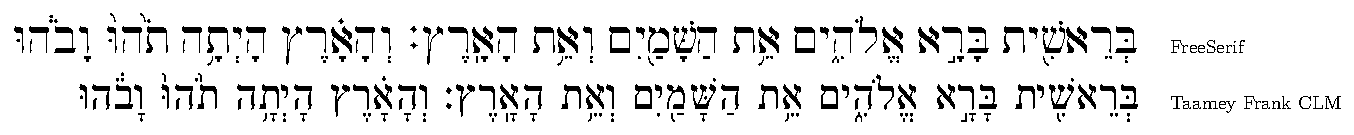
\includegraphics[width=\textwidth]{trop-fonts}
\caption{Genesis 1:1--2 in a general font and in a font made for trop.}
\label{fig:trop}
\end{figure}

So that nobody's source sheet is let down by its fonts without their knowing, the package
warns when a \texttt{mikra} source with trop is set in a font that isn't known to handle it,
unless you chose that font yourself with \cs{setshiurfont}. The warning appears once per
document, among \LaTeX's warnings, and says what to install. These fonts handle trop well,
and are free:
\begin{description}
\item[Ezra SIL] from SIL International (\url{https://software.sil.org/ezra/}); on Debian and
	Ubuntu, \texttt{sudo apt install fonts-sil-ezra}.
\item[Taamey Frank CLM] and Taamey David CLM, from the Culmus project
	(\url{https://culmus.sourceforge.io}).
\item[Keter YG] also from Culmus; on Debian and Ubuntu, \texttt{sudo apt install fonts-culmus}.
\item[SBL Hebrew] from the Society of Biblical Literature, free for non-commercial use.
\end{description}
For Rashi script, Noto Rashi Hebrew is part of Google's free Noto fonts.

\section{Sources of a text}

The companion package \texttt{teudot}, loaded with \verb|\usepackage{teudot}|, marks the
sources (strands) of a text, as in the documentary hypothesis, and shows each copy of a
\env{mekor} in colour, with some strands alone, or with the rest invisible but keeping their
space:
\begin{Verbatim}
\declareteudah[name=Yahwist]{j}{blue}
...
\begin{mekor}[\tanach{exodus}{14:19-23}]
\teudotsetup{show=j, others=omit}
\begin{mekorlang}{english}
\pasuk[14:19] \teudah{e} The angel of God moved. \teudah{j} The pillar ...
\end{Verbatim}
Verse numbers stay in place in every version. Its manual, \texttt{teudot-doc.pdf}, describes it.

\section{Other commands}

\begin{description}
\item[\cs{hdot}, \cs{Hdot}] \hdot\ and \Hdot, for transliteration (\Hdot anukah).
\item[\cs{sectionsymbol}] \sectionsymbol.
\item[\env{boxedtext}] text in a box, on handouts and slides.
\end{description}

\section{Licence}

Copyright 2023--2026 Gabriel Gendler Yom-Tov. This work may be distributed and/or modified
under the conditions of the \LaTeX\ Project Public License, either version 1.3c of this
license or (at your option) any later version.

\end{document}
